\section{Knowledge Graph}%
\label{sec:kgraph}
The \ac{hgraph} discussed in previous section has a lifetime that spans over a single task, learned system models are not stored for \ac{hgraph} that are created for future tasks. Storing learned environment knowledge is the \ac{kgraph}'s responsibility. Another responsibility of the \ac{kgraph} is to make an ordering in the stored environment knowledge. The ordering is made with a proposed success factor, a metric that combines multiple metrics such as prediction error, tracking error and the success-fail ratio of a edge parameterization (controller and system model).\bs

The name \quotes{\acl{kgraph}} originates from the environmental knowledge it contains, and its graph structure. Both the \ac{hgraph} and \ac{kgraph} are newly proposed methods build from the ground up, with only inspiration from an already existing technique, a backward search. The \ac{kgraph} does not adhere to any standard that may apply to standardized knowledge bases.\bs

\subsection{Definition}
\label{subsec:kgraph_definition}


\todo[inline]{this section}

\subsection{Edge Metrics}
\label{subsec:edge_metrics}
\subsection{Example}
\label{subsec:kgraph_example}



\subsection{Example}%
\label{subsec:kgraph_example}
An example \ac{kgraph} can be visualized in \Cref{fig:kgraph_example}, the parameterization of edges is displayed and the object that the edge controls as image. For clarification, the connected left part with image of the point robot on the center node has 3 outgoing edges that describe robot driving. The connected part on the right with an image of the point robot and the green box on the center node has 2 outgoing edges that describe robot pushing against the green box.\bs

\begin{figure}[H]
    \centering
    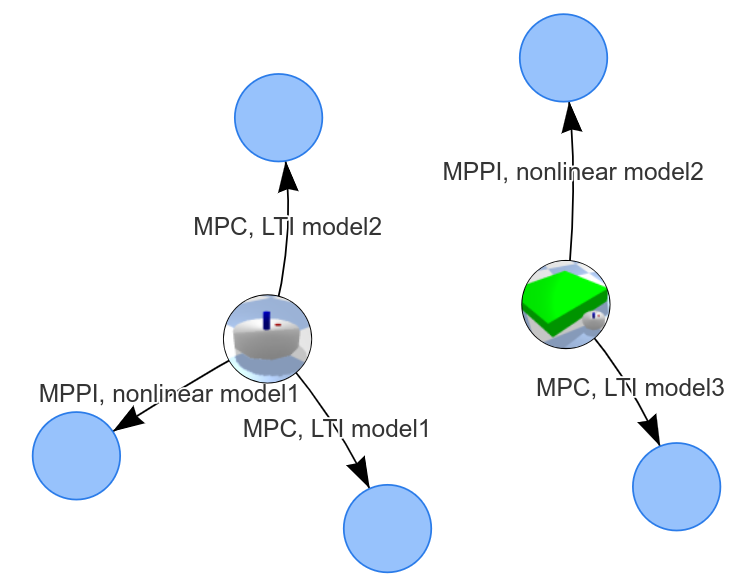
\includegraphics[width=10cm]{figures/kgraph_example}
    \caption{\ac{kgraph} with 3 edges on robot driving, and 2 edges for pushing the green box.}%
    \label{fig:kgraph_example}
\end{figure}

The edges in the figure above display only the edge parameterization, but store more information, mainly the success factor. The blue nodes serve a small purpose, making sure edges can point to a node. The blue nodes could fulfill a larger purpose, that is describing which actuators the edge can control. For example, a mobile robot with robot arm attached can have a set of controllers that only drive the base, a set of controllers that only steer the robot arm and a set that controls both the base and robot arm. In such cases the blue nodes describe which part can of the robot can be actuated. The controllers considered in this thesis control every actuator of the robot, resulting in the blue nodes serving such a small purpose.\bs

\subsection{Edge Metrics}%
\label{subsec:edge_metrics}
The \ac{kgraph} keeps an ordered list of `good' and `bad' edge arguments (controller and system model). `Good' and `bad' are defined by edge metrics, these metrics are created after the completion of an edge, regardless of whether the edge was successfully completed or failed. An indication is given on why certain metrics matter in \cref{table:review_edge_metrics}.

\noindent
\begin{table}[H]
\centering
\begin{tabular}%
{>{\raggedright\arraybackslash}p{0.25\textwidth}%
>{\raggedright\arraybackslash}p{0.65\textwidth}}
\acf{PE}&  To better compare prediction errors the \ac{PE} is summarised and average \ac{PE}. The average \ac{PE} is an indicator of an accurate system model but can give misleading results since \ac{PE} is also an indicator of unexpected collisions. Prediction error should thus only be used if there are no collisions detected. The average \ac{PE} comes with more flaws since the average is mostly determined by outliers, some unfortunate outliers in the \ac{PE} might for the largest part determine the average \ac{PE}. The average \ac{PE} will thus not be used because it is not robust enough.\\
\acf{TE}& For a low \ac{TE} the system model must be close to the real motion equations to yield a feasible path, the controller must be well tuned to be able to track that path and the controller and system model must be in collaboration, because the controller uses the system model to calculate system input. A low \ac{TE} tells multiple things, whilst a high \ac{TE} would indicate improvements could be gained in the controller, the system model or their collaboration.\\
ratio num\_succesfully completed edges and num\_total edges & Over time the \ac{kgraph} can recommend the same edge arguements multiple times. Logging the ratio of succeeding edges vs total edges builds an evident portfolio. Still, this metric has to be taken with a grain of salt because edges with equal edge arguments perform similar actions e.g.~pushing an object through a wide corridor is compared to pushing the same object through a narrow corridor. One could say \quotes{comparing apples with pears}.\\
the final position and \newline displacement error & The quality of the result is measured in the final position and displacement error. The importance should thus be stressed when ordering edge arguments.\\
planning time& With system identification, path estimation, motion or manipulation planning the planning time can vary in orders of magnitude between simple or more complex approaches. Planning time mainly serves to rank the slowest planners low, whilst not influencing the rank of fast and average planners.\\
runtime& Also known as execution time would be a quality indicator if start and target states would be equal. Edges are recommended to solve similar tasks, where the path length between the start and target state is different. Thus planning time is not of any use to rank edges.\\
completion time = \newline runtime + planning time & With the same arguementation as runtime, completion time is not of any use to rank edges.\\
\end{tabular}
\caption{Edge metrics used to rank control methods from `good' to `bad'}
\label{table:review_edge_metrics}
\end{table}


The \ac{kgraph} fulfills two goals. It stores information whether an object an be manipulated, and stores an ordered list from most successful control and system model combination to least successful per object. Information if objects can be manipulated prevent hypothesis from trying to push unmovable objects. A list of most successful control and system model combinations will suggest the best possible combination to fulfill the drive of pushing action.\bs

